\section{Algoritmo de consenso Prueba de Devoción (\textit{Proof of Devotion}, PoD)}
\label{sec:pod}

\subsection{Metas de diseño}
\label{pod:goals}

The consensus algorithm is one of the cornerstones of blockchains, and its rapidity and irreversibility are our focus. In addition, in order to build a good ecology of Nebulas, we believe that fairness is equally important. If the big capital can easily gain power to control the block consensus in Nebulas, the interests of many developers and users will be damaged. It is difficult for an ecology which cannot guarantee the interests of contributors to create in-depth value, as it goes against the design principles of Nebulas. Thus, the consensus algorithm should be designed to ensure the rapidity and irreversibility first, on which basis we will pursue fairness as much as possible, so as to guarantee the interests of contributors in Nebulas.

\subsection{Defects of Commonly Used Consensus Algorithms}
\label{pod:weakness}

We have tried to find suitable commonly used consensus algorithms that match with our design goals, but these algorithms cannot completely meet our requirements.

The PoW (Proof of Work) consensus algorithm is a zero-sum game, which uses the competitive hash calculation to determine the bookkeeper, rendering a great amount of electric power in the whole ecology wasted in the competition when any blocks are fed out, and thus the mining cost is high and the speed is restricted. With the increase of nodes involved in mining, the probability of each node to obtain the bookkeeping right will be reduced, leading to a continuous rise in the cost of stable feed-out of blocks under the PoW protocol. The Bitcoin, which continues to increase the difficulty of mining, has to face the situation sooner or later where the mining machine cannot make ends meet, while Ethereum has long been considering the use of the new PoS consensus algorithm Casper \cite{casper} to gradually replace the current PoW consensus \cite{buterin2013ethereum}. It can be seen that in view of the mining speed and the economic cost, the PoW is not beneficial to the long-term rapid development of the ecology of Nebulas, which is against our ``rapid" goals.

The PoS (Proof of Stake) consensus algorithm attempts to use the asset amount to replace the hash rate and distribute the probability of obtaining the bookkeeping right according to the coin age or deposit amount. Currently, both Peercoin \cite{king2012peercoin} and the Casper Protocol of Ethereum adopt the PoS consensus algorithm. This algorithm overcomes the shortcoming of the high power consumption of PoW but visually enlarges the impact of the capital on the probability distribution of the bookkeeping right. Compared with PoW, the big capital under PoS is more likely to gain power to control the ecology and form large group monopoly, possibly damaging the interests of the ecology contributors and impacting adversely on the value generation of Nebulas, all of which are against our ``fairness" goal.

The PoI (Proof of Importance) consensus algorithm was first proposed by Nem \cite{nem}. Different from PoS, the concept of account importance is introduced to PoI, and the account importance score is used to distribute the probability of the bookkeeping right. This algorithm overcomes the shortcoming of the high power consumption of PoW and relieves the PoS capital monopoly crisis, but exposes the ``nothing-at-stake" problem. The cost for a cheater to reverse a block is significantly reduced, which goes against our ``irreversibility" goal.

In short, in view of the discrepancy between commonly used consensus algorithms and our goals, we have proposed the PoD (Proof of Devotion) algorithm to integrate PoI, which evaluates the comprehensive account influence, with PoS, which involves strict economic penalties. PoS enhances the irreversibility of PoI, while PoI reversely contains the monopoly of PoS, which facilitates the free and rapid development of the ecology.

\subsection{Design of the PoD Algorithm}
\label{pod:design}

\subsubsection{Generation of New Blocks}
\label{pod:design:block}

Similar to the PoI consensus algorithm that selects highly important accounts, the PoD selects the accounts with high influence in the ecology. The difference lies in that the PoD empowers the selected accounts to have the bookkeeping right with equal probability to participate in new block generation in order to prevent tilted probability that may bring about monopoly.

When selecting accounts with high influence, we use NR, the universal measure of value generated from Nebulas. In the algorithm design of NR, we highlighted the liquidity and propagation of accounts (see \refsec{subsec:value}). We believe that the accounts featured with these properties have a high influence with regard to the ecology construction. Thus, in the PoD, the accounts ranked Top N in the NR will be selected, and after these accounts voluntarily pay a certain number of NASs as the deposit, they will be qualified as the validator of new blocks to participate in bookkeeping.

After the validator set is provided, the PoD algorithm uses the pseudo-random number to determine which one in the set is the new block proposer, which need to pack recent transactions to generate the new block. The validator set is changeable. The eligible account can choose to join or quit the set. Besides, the eligible accounts may vary with the periodical change of NR. Therefore, we designed the dynamic validator set change mechanism in the PoD to implement the change of the validator set.

\subsubsection{Dynamic Validators Set}
\label{pod:design:validators}

The validator set changes the same way as a dynasty, so the set is divided into different dynasties, and the validator set within a dynasty will not change. A dynasty cannot experience too rapid change, and no change should be made within a period of time. Thus, we define every X blocks as an Epoch, and in the same Epoch, no change takes place in the dynasty. Therefore, the change of dynasties will only occur when one Epoch is handed over to another. At that time, the first block of the previous Epoch will be investigated. If this block reaches the finality state, then the current Epoch will enter into the next dynasty of D1; otherwise, the previous dynasty of D0 will remain; the process of which is shown in \reffig{fig:epoch}.

\begin{figure}[h]
\centering
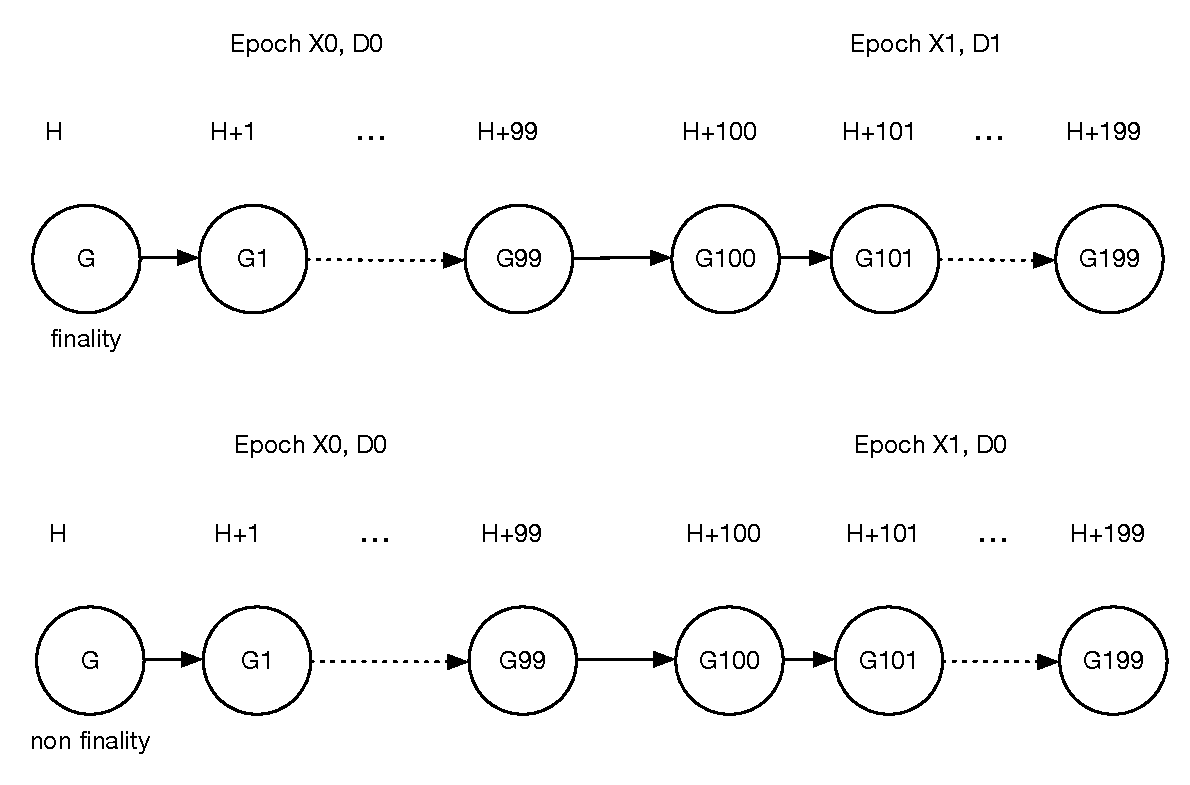
\includegraphics[width=8cm]{./figs/epoch}
\caption{Change of validator dynasties (assuming X = 100)}
\label{fig:epoch}
\end{figure}

Because of the network delay, the finality state of Block G at each node may not be the same when any change of dynasties takes place. Therefore, by reference to dynamic Casper validator set strategies, it is required that the consensus process of each dynasty will be completed jointly by the validator sets of the current and previous dynasties. Therefore, in any dynasty, an eligible account can only apply for joining or quiting the validator set of Dynasty D+2, and when the dynasty evolves into Dynasty D+2, it can participate in the consensus process of the new block.

\subsubsection{Consensus Process}
\label{pod:design:consensus}

After a new block is proposed, all the people in the validator set of the current dynasty will participate in a round of BFT-Style (Byzantine-Fault-Tolerant Style) voting to determine the legitimacy of this block. In the beginning of voting, each validator who participates in this block consensus will be charged 2x (x is the incentive bonus proportion) as the deposit and then the two-stage voting process will be kicked off.

\begin{itemize}

\item \textbf{In the first stage}, it is required that all validators vote $Prepare$ tickets for the new block. After voting the $Prepare$ ticket, the validator will be rewarded $1.5x$ bonus. If the validators holding over two-thirds of the total deposits in both current and previous dynasties vote $Prepare$ tickets for the new block, this block will enter into the second stage of voting. It should be noted that the proposer of the new block votes the $Prepare$ ticket for the new block by default.

\item \textbf{In the second stage}, it is required that all validators vote $Commit$ tickets for the new block. After voting the $Commit$ ticket, the validator will be rewarded $1.5x$ bonus again. If the validators holding over two-thirds of the total deposits in both current and previous dynasties vote $Commit$ tickets for the new block, this block will reach the finality state.
\end{itemize}

In order to speed up the development of the entire ecology, if the difference between the timestamp of $Prepare$ ticket and $Commit$ ticket in Block b and the timestamp of Block b exceeds $T$, then these tickets will be considered expired and will be ignored directly.

\subsubsection{Fork Choice}
\label{pod:design:fork}

The PoD algorithm selects the canonical chain according to the block score at each height. It always selects the block with the highest score to join the canonical chain, and the score of Block b at Height h is as follows:

\begin{align}
Score(b, h) = \sum_{(b',h') \in children(b)}Score(b', h') + \sum committed~deposits~in~b
\end{align}
\noindent

Namely the sum of deposits corresponding to $Commit$ tickets received by this block and all of its descendant blocks, as shown in \reffig{fig:fork_choice}.

\begin{figure}[h]
\centering
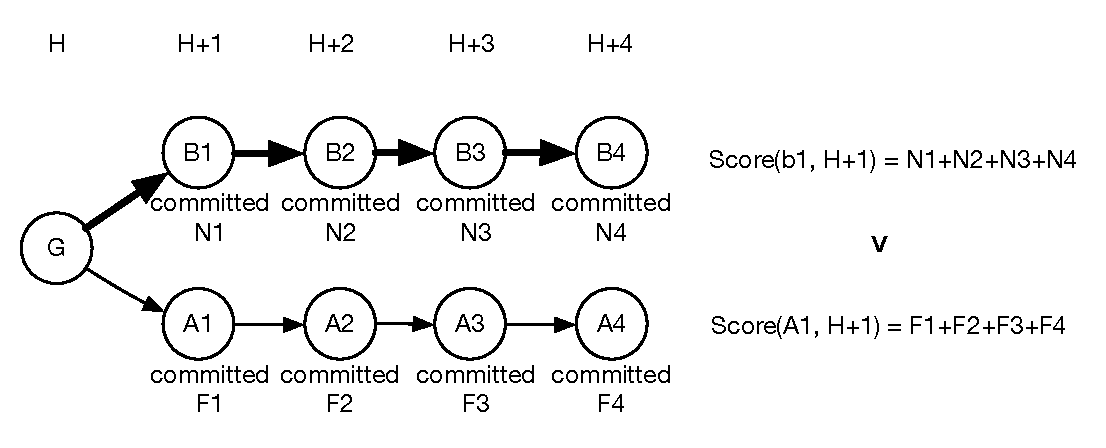
\includegraphics[width=12cm]{./figs/fork}
\caption{Fork Choice Example}
\label{fig:fork_choice}
\end{figure}

\subsubsection{Slashing Conditions}
\label{pod:design:vote}

To avoid any malicious damage to the consensus process, which may result in failure in the completion of consensus process and obstruction of eco-development, PoD constrains consensus activities of validators based on reference to Casper’s minimum slashing conditions \cite{minimal_slash_rules}.

Assume that $Prepare$ vote and $Commit$ vote in the consensus process have the following structures:

\begin{itemize}
\item $Prepare(H, v, vs)$, where $H$ is the hash value of the current block; $v$ represents the height of the current block; $vs$ represents the height of a certain ancestral block of $v$.

\item $Commit(H, v)$, where $H$ is the hash value of the current block; $v$ represents the height of the current block.
%\item $Commit(H, v)$,其中H为当前区块hash,$v$表示当前区块高度
\end{itemize}

PoD algorithm defines the following 4 basic rules for the entire voting process:

\begin{itemize}
\item There is a strict order in the two-stage consensus process of a single block: Only when the total deposits of $Prepare(H, v, vs)$ votes for the first stage reaches $2/3$, can validators deliver $Commit(H, v)$ votes for the second stage.

\item For multiple blocks, there is no mandatory rule that only when the consensus process of one block is finished, may consensus process of the next block begin. Interwoven consensus is permitted providing that it is conducted based on a certain order. Only after the first stage of process for height vs is finished and the proportion of $Prepare(H, vs, vs’)$ votes reaches $2/3$, can $Prepare(H, v, vs)$ votes for its descendant blocks be delivered based on vs in order to ensure stable proceeding of the interwoven consensus.

\item To avoid the conduct of malicious cross-block voting of any node by taking advantage of the interwoven consensus, it is required that after the delivery of Prepare (H, w, u) votes based on the height of u, no Commit(H, v) vote can be delivered in all blocks with a height within the range from u to w, thus guaranteeing high efficiency and orderliness of the consensus process.

\item For the purpose of preventing nodes from staking with one deposit on multiple branches simultaneously, which may lead to the problem of “nothing-at-stake”, it is required that after $Prepare(H1, v, vs1)$ votes are delivered at a certain height, no different $Prepare(H2, v, vs2)$ vote can be delivered again.
\end{itemize}

Once being reported and verified, any validators breaking the above rules will be punished and all his/her deposit will be confiscated, in which 4\% will be shared by whistleblowers as a reward and the remaining part will be destroyed.

\subsection{PoD Economic Analysis}
\label{pod:economic}

\subsubsection{Incentive Analysis}
\label{pod:economic:incentive}

A validator participating in the PoD algorithm will be rewarded with $1x$ NAS on each legal block. In case of failure in finishing the $Prepare$ stage and entering into the $Commit$ stage due to poor network traffic or any cheating behavior, the validator will lose $0.5x$ NAS. Therefore, any validator becoming value nodes will secure a large amount of earnings from accounting under good network traffic when not engaging in any cheating behavior.

\subsubsection{Cheating Analysis}
\label{pod:economic:fraud}

\subsubsection*{Double-spend Attack}
\label{pod:economic:fraud:double_spend}

If it is assumed that a merchant confirms transaction and makes delivery when the new block reaches the status of finality, then the minimum cost to be paid by a fraud for realizing zero-cost shopping through completion of double-spend attack under the PoD consensus algorithm is described as follows:

Firstly, the fraud needs to increase his/her Nebulas Rank to Top N, become a validator by paying a certain amount of NAS as deposit and apply for participation in validation of blocks in the D+2 dynasty.

Then, the fraud needs to be selected as the proposer of a new block by the pseudo-random algorithm. At this moment, the fraud proposes two new blocks at the same height, of which one block has a hash value of hash1 and contains a transferring transaction from the fraud to the merchant, while the other block has a hash value of hash2 and contains a transferring transaction from the fraud to himself/herself.

Finally, in order to make both of hash1 and hash2 blocks reach finality, as shown in \reffig{fig:double_spend}, the fraud has to spend $1/3$ of the total deposits in this dynasty to bribe $1/3$ of the validators and make them to deliver $Commit$ votes to both blocks.

\begin{figure}[h]
\centering
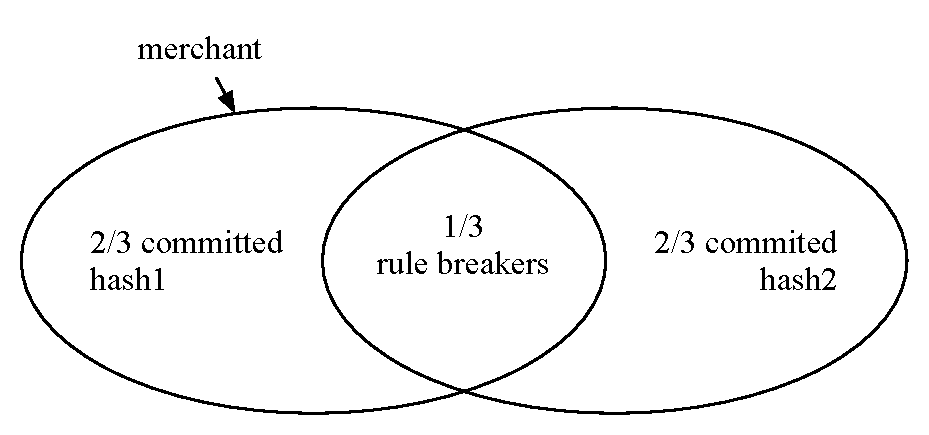
\includegraphics[width=7cm]{./figs/overlap}
\caption{Financial Punishment on Double Spend}
\label{fig:double_spend}
\end{figure}

Therefore, in order to complete a successful double-spend attack, the fraud needs to spend a certain amount of energy and financial resource to increase his/her Nebulas Rank (see \refsec{subsec:robust} Resistance to Manipulation) and then spend at least $1/3$ of the total deposits in current dynasty to make both of the blocks reach the finality status after he/she is luckily selected as a proposer.

\subsubsection*{51\% attack}
\label{pod:economic:fraud:51attack}

In PoW, launch of a 51\% attack requires 51\% of hashrate. In PoS, launch of a 51\% attack requires 51\% of deposit. However, in PoD, launch of a 51\% attack requires 51\% of accounts in the validators set, which means that a sufficient number of highly-reputed users need to rank at Top N in the Nebulas Rank and payment of a corresponding amount of deposit is required, so it will be more difficult to launch a 51\% attack in PoD.

\subsubsection*{Short-range Attack}
\label{pod:economic:fraud:short_range_attack}

In PoD, blocks at each height have term of expiration time of consensus. Therefore, it is almost impossible to complete a long-range attack in PoD, but it is still possible to launch short-range attacks within term of expiration time.

When a short-range attacker (Attacker) attempts to forge A-chain to replace B-chain to become the canonical fork when blocks at the height of H+1 are still within term of expiration time, Attacker needs to ensure that score of block A1 is higher than that of block B1. Multiple voting will be severely punished, so it will be unavoidable for Attacker to bribe validators; otherwise, it is impossible to complete a short-range attack. For the purpose of presenting the safety of the PoD consensus algorithm, the costs to be paid by Attacker in reverting different numbers of blocks are analyzed as follows.

If Attacker plans to revert B1, the minimum cost to be paid by Attacker is as described in \reffig{fig:revert1}, which is equivalent to a double-spend attack. If Attacker becomes the proposer of blocks at the height of H+1, then he/she has to bribe $1/3$ of the validators in Dynasty D0 and make them conduct multiple voting in order to make A1 reach finality, for which the minimum cost is $1/3$ of the total deposits.

\begin{figure}[h]
\centering
\includegraphics[width=11cm]{./figs/revert1}
\caption{Revert One Block by Short-range Attack}
\label{fig:revert1}
\end{figure}

Assume that B1 and B2 have reached the status of finality and transactions in the blocks have come into effect. If Attacker wants to revert B1-B2, the following two circumstances are taken into consideration.

\begin{itemize}
\item The first circumstance is shown in Figure \ref{fig:revert2} (a): When Heights H+1 and H+2 are in the same Epoch and dynasty, Attacker needs to bribe $1/3$ of the validators in D0 in order to make A1 reach finality. Meanwhile, these $1/3$ of the validators will be punished and their deposits will be totally confiscated. During validation of A2, sum of deposits equals to $2/3$ of deposits in A1. At this moment, if Attacker wants to secure the same amount of commit votes as B2, he/she has to bribe all the remaining validators without cheating and lose at least $3/3$ of the total deposits. Even if Attacker succeeds in doing this, it is impossible to guarantee that score of A1 is higher than that of B1 and Attacker will face a high risk of failure of attack.

\item The second circumstance is shown in Figure \ref{fig:revert2} (b): When Heights H+1 and H+2 are in different Epochs and different dynasties, Attacker needs to bribe $1/3$ of the validators in D0 to make A1 reach finality and then bribe $1/3$ of the validators in D1 to make A2 reach finality, so Attacker will lose at least $2/3$ of the total deposits in order to complete such an attack. To sum up, to launch a short-range attack to cause invalidation of two blocks that have reached finality, Attacker needs to pay at least $2/3$ of the total deposits.
\end{itemize}

\begin{figure}[h]
\centering
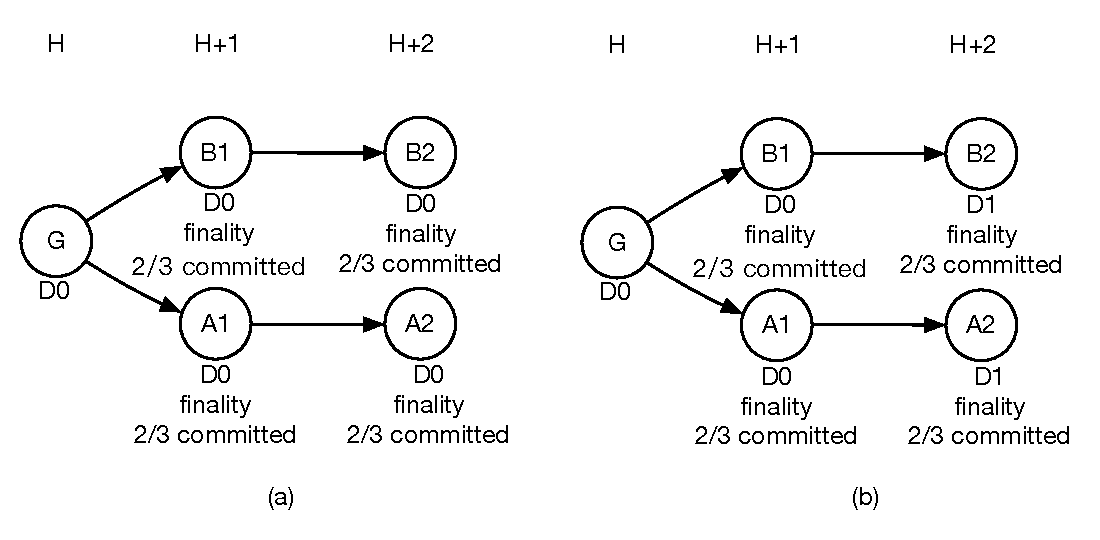
\includegraphics[width=11cm]{./figs/revert2}
\caption{Revert Two Blocks by Short-range Attack}
\label{fig:revert2}
\end{figure}

If Attacker wants to revert B1-B3, as shown in Figure 18, Attacker needs to firstly bribe $1/3$ of the validators in D0 in order to realize finality of A1 and then bribe $1/3$ of the validators in D1 in order to realize finality of A2. Finally, Attacker needs to bribe all of the remaining $2/3$ of the validators in D1 in order to realize finality of A3. To sum up, $4/3$ of the total amount of deposits will be lost. It will be very difficult to prepare for these attacks. Even if an attacker manages to succeed in making necessary preparations, he/she can’t guarantee that score of A1 is higher than that of B1. Therefore, it is possible that such attack may fail.

\begin{figure}[h]
\centering
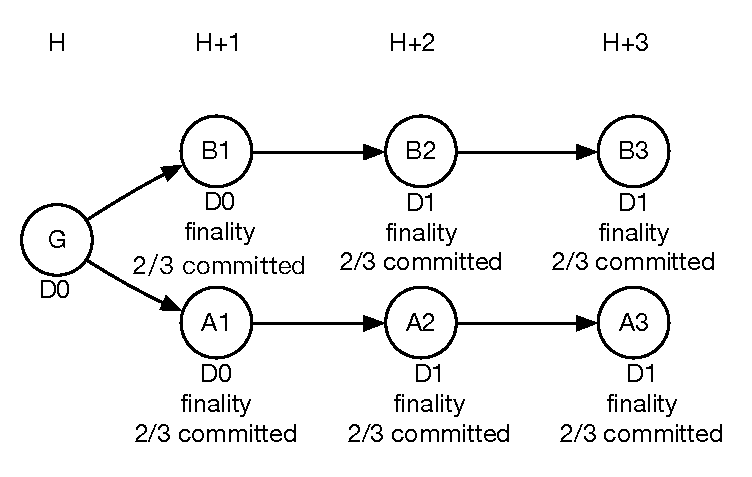
\includegraphics[width=7.5cm]{./figs/revert3}
\caption{Revert Three Blocks by Short-range Attack}
\label{fig:revert3}
\end{figure}

If Attacker wants to revert B1-BN, in which N is limited by term of expiration time of consensus of the block and thus can't be a very large number. When $N = 3$, the total deposits of all validators in the current dynasty will be totally confiscated. Therefore, when $N >= 4$, it is impossible to complete an attack in order to make score of B1 higher than that of A1 and revert B1-BN. It is pointless to launch such an attack.